% Thinking in Documents
% (c) Copyleft 2010. 
% Cesar Rodas 
%
% Based on http://www.cs.berkeley.edu/~mdw/proj/texslides for details.

\documentclass[20pt,landscape]{foils}
\usepackage{eso-pic}
\usepackage{mdwslides}

\usepackage[english]{babel}
\hypersetup{
  pdfmenubar=false,
  pdftoolbar=false,
  colorlinks=true,
  urlcolor=mygreen,
  pdfpagemode={None},
  pdftitle={MongoDB and PHP},
  pdfauthor={Cesar D. Rodas},
  pdfsubject={},
  pdfkeywords={PHP, MongoDB}
}

\usepackage{hyperref}
\usepackage{pause}
\usepackage{graphicx}


%%%%%%%%%%%%%%%%%%%%%%%%%%%%%%%%%%%%%%%%%%%%%%%%%%%%%%%%%%%%%%%%%%%%%%%%%%%%
% Fondo
%%%%%%%%%%%%%%%%%%%%%%%%%%%%%%%%%%%%%%%%%%%%%%%%%%%%%%%%%%%%%%%%%%%%%%%%%%%%
%\definecolor{bg2}{rgb}{1,1,1}
\definecolor{bg2}{rgb}{1, 0.99, 0.99}
\definecolor{bg1}{rgb}{0.99, 0.99, 0.5}
\definecolor{mygreen}{rgb}{0,0.4,0}
\vpagecolor[bg1]{bg2}

%%%%%%%%%%%%%%%%%%%%%%%%%%%%%%%%%%%%%%%%%%%%%%%%%%%%%%%%%%%%%%%%%%%%%%%%%%%%
% Set headers
%%%%%%%%%%%%%%%%%%%%%%%%%%%%%%%%%%%%%%%%%%%%%%%%%%%%%%%%%%%%%%%%%%%%%%%%%%%%
\MyLogo{\color{mdwblue}\href{http://twitter.com/crodas}{@crodas} - \href{http://crodas.org}{http://cesarodas.com/} - \LaTeX}
\rightfooter{\quad\textsf{\thepage}}

\begin{document}
\rm

%%%%%%%%%%%%%%%%%%%%%%%%%%%%%%%%%%%%%%%%%%%%%%%%%%%%%%%%%%%%%%%%%%%%%%%%%%%%
% Presentacion
%%%%%%%%%%%%%%%%%%%%%%%%%%%%%%%%%%%%%%%%%%%%%%%%%%%%%%%%%%%%%%%%%%%%%%%%%%%%
\slide{}
\LogoOff

\vskip 3in
\begin{center}
{\color{mdwblue}\huge\trebucbd  MongoDB and PHP}

\vskip 5ex
C�sar D. Rodas\\
{\small\trebucit \href{mailto:crodas@ferpectos.com}{crodas@ferpectos.com}}\\
{\mdwsmall\tt \href{http://cesarodas.com/}{http://cesarodas.com/}}\\
    \vskip 5ex

\vskip 1ex
Latinoware 2010\\
    Foz do Igua�u, Brasil\\
\end{center}

%%%%%%%%%%%%%%%%%%%%%%%%%%%%%%%%%%%%%%%%%%%%%%%%%%%%%%%%%%%%%%%%%%%%%%%%%%%%
% Who am I?
%%%%%%%%%%%%%%%%%%%%%%%%%%%%%%%%%%%%%%%%%%%%%%%%%%%%%%%%%%%%%%%%%%%%%%%%%%%%
\slide{Who is this fellow?}
\LogoOn

\begin{list1}
    \item Paraguayan :-)
    \item Zealot of
    \begin{list2}
        \item Open Source (BSD-license)
        \item PHP
        \item MongoDB
    \end{list2}
    \item PECL Developer
    \item Work for a \href{http://www.plumwillow.com/plum/team}{cool company} (btw, we're hiring)
    \item \href{http://www.cesarodas.com/}{... and few other things}

\end{list1}

%%%%%%%%%%%%%%%%%%%%%%%%%%%%%%%%%%%%%%%%%%%%%%%%%%%%%%%%%%%%%%%%%%%%%%%%%%%%
% Agenda
%%%%%%%%%%%%%%%%%%%%%%%%%%%%%%%%%%%%%%%%%%%%%%%%%%%%%%%%%%%%%%%%%%%%%%%%%%%%
\slide{Agenda}

\begin{list1}
    \item Introduction to MongoDB
    \item MongoDB Queries
    \item Real life example:
        \begin{list2}
            \item Designing data model for a Wordpress.com like site
            \item Optimize our data model to run in sharded environment
        \end{list2}
\end{list1}

%%%%%%%%%%%%%%%%%%%%%%%%%%%%%%%%%%%%%%%%%%%%%%%%%%%%%%%%%%%%%%%%%%%%%%%%%%%%
% MongoDB
%%%%%%%%%%%%%%%%%%%%%%%%%%%%%%%%%%%%%%%%%%%%%%%%%%%%%%%%%%%%%%%%%%%%%%%%%%%%
\slide{MongoDB}

\begin{list1}
    \item <EN>Mongo</EN> != <PT>Mongo</PT>
    \item Document oriented database
    \item Fast, Scalable, Easy to use (devel-friendly)
    \item Support Indexes 
    \begin{list2}
        \item Simple
        \item Compound 
        \item Geo spatial
    \end{list2}
    \item Schemaless
    \item Support sharding
    \item Nested documents
    \item PECL client 
\end{list1}

%%%%%%%%%%%%%%%%%%%%%%%%%%%%%%%%%%%%%%%%%%%%%%%%%%%%%%%%%%%%%%%%%%%%%%%%%%%%
% 
%%%%%%%%%%%%%%%%%%%%%%%%%%%%%%%%%%%%%%%%%%%%%%%%%%%%%%%%%%%%%%%%%%%%%%%%%%%%
\slide{}

\vskip 4in
\begin{center}
    {\color{mdwblue}\Huge\trebucbd Documents?}
\end{center}


%%%%%%%%%%%%%%%%%%%%%%%%%%%%%%%%%%%%%%%%%%%%%%%%%%%%%%%%%%%%%%%%%%%%%%%%%%%%
% 
%%%%%%%%%%%%%%%%%%%%%%%%%%%%%%%%%%%%%%%%%%%%%%%%%%%%%%%%%%%%%%%%%%%%%%%%%%%%
\slide{}

\vskip 4in
\begin{center}
    {\color{mdwblue}\Huge\trebucbd It's just an Array()}
\end{center}

%%%%%%%%%%%%%%%%%%%%%%%%%%%%%%%%%%%%%%%%%%%%%%%%%%%%%%%%%%%%%%%%%%%%%%%%%%%%
% 
%%%%%%%%%%%%%%%%%%%%%%%%%%%%%%%%%%%%%%%%%%%%%%%%%%%%%%%%%%%%%%%%%%%%%%%%%%%%
\slide{}

\vskip 4in
\begin{center}
    {\color{mdwblue}\Huge\trebucbd In fact everything is an Array() in MongoDB}
\end{center}

%%%%%%%%%%%%%%%%%%%%%%%%%%%%%%%%%%%%%%%%%%%%%%%%%%%%%%%%%%%%%%%%%%%%%%%%%%%%
% 
%%%%%%%%%%%%%%%%%%%%%%%%%%%%%%%%%%%%%%%%%%%%%%%%%%%%%%%%%%%%%%%%%%%%%%%%%%%%
\slide{}
\vskip 4in
\begin{center}
    {\color{mdwblue}\Huge\trebucbd \href{http://bit.ly/mongodb-php}{http://bit.ly/mongodb-php}}
\end{center}

%%%%%%%%%%%%%%%%%%%%%%%%%%%%%%%%%%%%%%%%%%%%%%%%%%%%%%%%%%%%%%%%%%%%%%%%%%%%
% 
%%%%%%%%%%%%%%%%%%%%%%%%%%%%%%%%%%%%%%%%%%%%%%%%%%%%%%%%%%%%%%%%%%%%%%%%%%%%
\slide{}

\vskip 4in
\begin{center}
    {\color{mdwblue}\Huge\trebucbd Documents?}
\end{center}


%%%%%%%%%%%%%%%%%%%%%%%%%%%%%%%%%%%%%%%%%%%%%%%%%%%%%%%%%%%%%%%%%%%%%%%%%%%%
% 
%%%%%%%%%%%%%%%%%%%%%%%%%%%%%%%%%%%%%%%%%%%%%%%%%%%%%%%%%%%%%%%%%%%%%%%%%%%%
\slide{}

\vskip 4in
\begin{center}
    {\color{mdwblue}\Huge\trebucbd It's just an Array()}
\end{center}

%%%%%%%%%%%%%%%%%%%%%%%%%%%%%%%%%%%%%%%%%%%%%%%%%%%%%%%%%%%%%%%%%%%%%%%%%%%%
% 
%%%%%%%%%%%%%%%%%%%%%%%%%%%%%%%%%%%%%%%%%%%%%%%%%%%%%%%%%%%%%%%%%%%%%%%%%%%%
\slide{}

\vskip 4in
\begin{center}
    {\color{mdwblue}\Huge\trebucbd In fact everything is an Array() in MongoDB}
\end{center}

%%%%%%%%%%%%%%%%%%%%%%%%%%%%%%%%%%%%%%%%%%%%%%%%%%%%%%%%%%%%%%%%%%%%%%%%%%%%
% 
%%%%%%%%%%%%%%%%%%%%%%%%%%%%%%%%%%%%%%%%%%%%%%%%%%%%%%%%%%%%%%%%%%%%%%%%%%%%
\slide{}
\vskip 4in
\begin{center}
    {\color{mdwblue}\Huge\trebucbd \href{http://bit.ly/mongodb-php}{http://bit.ly/mongodb-php}}
\end{center}

%%%%%%%%%%%%%%%%%%%%%%%%%%%%%%%%%%%%%%%%%%%%%%%%%%%%%%%%%%%%%%%%%%%%%%%%%%%%
% 
%%%%%%%%%%%%%%%%%%%%%%%%%%%%%%%%%%%%%%%%%%%%%%%%%%%%%%%%%%%%%%%%%%%%%%%%%%%%
\slide{MongoDB - Operations}

\begin{list1}
    \item Select
    \begin{list2}
        \item \$gt, \$lt, \$gte, \$lte, \$eq, \$neq: >, <, >=, <=, ==, !=
        \item \$in, \$nin, \$or
        \item \$size, \$exists
        \item \$where: Any javascript expression
        \item group()
        \item limit()
        \item skip()
    \end{list2}
    \item Update
    \begin{list2}
        \item \$set
        \item \$unset
        \item \$push
        \item \$pull
        \item \$inc
        \item findAndModify()
    \end{list2}
\end{list1}



%%%%%%%%%%%%%%%%%%%%%%%%%%%%%%%%%%%%%%%%%%%%%%%%%%%%%%%%%%%%%%%%%%%%%%%%%%%%
% 
%%%%%%%%%%%%%%%%%%%%%%%%%%%%%%%%%%%%%%%%%%%%%%%%%%%%%%%%%%%%%%%%%%%%%%%%%%%%
\slide{}

\vskip 4in
\begin{center}
    {\color{mdwblue}\Huge\trebucbd Is it better than my MySQL (or Pg)?}
\end{center}

%%%%%%%%%%%%%%%%%%%%%%%%%%%%%%%%%%%%%%%%%%%%%%%%%%%%%%%%%%%%%%%%%%%%%%%%%%%%
% 
%%%%%%%%%%%%%%%%%%%%%%%%%%%%%%%%%%%%%%%%%%%%%%%%%%%%%%%%%%%%%%%%%%%%%%%%%%%%
\slide{}

\vskip 4in
\begin{center}
    {\color{mdwblue}\Huge\trebucbd NO.}
\end{center}

%%%%%%%%%%%%%%%%%%%%%%%%%%%%%%%%%%%%%%%%%%%%%%%%%%%%%%%%%%%%%%%%%%%%%%%%%%%%
% 
%%%%%%%%%%%%%%%%%%%%%%%%%%%%%%%%%%%%%%%%%%%%%%%%%%%%%%%%%%%%%%%%%%%%%%%%%%%%
\slide{}

\vskip 4in
\begin{center}
    {\color{mdwblue}\Huge\trebucbd It is different.}
\end{center}

%%%%%%%%%%%%%%%%%%%%%%%%%%%%%%%%%%%%%%%%%%%%%%%%%%%%%%%%%%%%%%%%%%%%%%%%%%%%
% 
%%%%%%%%%%%%%%%%%%%%%%%%%%%%%%%%%%%%%%%%%%%%%%%%%%%%%%%%%%%%%%%%%%%%%%%%%%%%
\slide{Differences with a rel. database}

\begin{list1}
    \item Denormalize data is not bad
    \begin{list2}
        \item It makes queries simplest and faster
        \item Disk-space is much cheaper than CPU (and your user's time)
        \item Much simple to distribute data across multiple nodes
    \end{list2}
    \item No CPU wasting doing ORM
    \begin{list2}
        \item Objects in the programming language and in the database
        \item No abstraction to generate SQL
    \end{list2}
    \item No SQL injection :-)
    \item No Joins (they are evil!)
    \item Batch processing
    \item No CREATE TABLE (or ALTER TABLE) needed
\end{list1}

%%%%%%%%%%%%%%%%%%%%%%%%%%%%%%%%%%%%%%%%%%%%%%%%%%%%%%%%%%%%%%%%%%%%%%%%%%%%
% 
%%%%%%%%%%%%%%%%%%%%%%%%%%%%%%%%%%%%%%%%%%%%%%%%%%%%%%%%%%%%%%%%%%%%%%%%%%%%
\slide{}
\vskip 1in
\begin{center}
    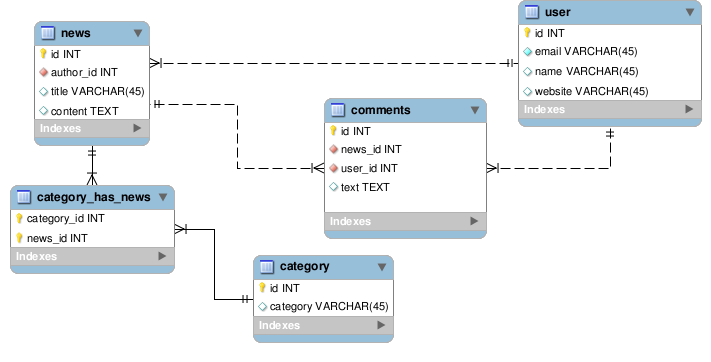
\includegraphics{relation.png}
\end{center}

%%%%%%%%%%%%%%%%%%%%%%%%%%%%%%%%%%%%%%%%%%%%%%%%%%%%%%%%%%%%%%%%%%%%%%%%%%%%
% 
%%%%%%%%%%%%%%%%%%%%%%%%%%%%%%%%%%%%%%%%%%%%%%%%%%%%%%%%%%%%%%%%%%%%%%%%%%%%
\slide{}
\vskip 4in
\begin{center}
    {\color{mdwblue}\Huge\trebucbd The fun part}
\end{center}

%%%%%%%%%%%%%%%%%%%%%%%%%%%%%%%%%%%%%%%%%%%%%%%%%%%%%%%%%%%%%%%%%%%%%%%%%%%%
% 
%%%%%%%%%%%%%%%%%%%%%%%%%%%%%%%%%%%%%%%%%%%%%%%%%%%%%%%%%%%%%%%%%%%%%%%%%%%%
\slide{Data-structure}

\vskip -0.1in
\definecolor{000000}{rgb}{0.000,0.000,0.000}
\definecolor{0000BB}{rgb}{0.000,0.000,0.733}
\definecolor{007700}{rgb}{0.000,0.467,0.000}
\definecolor{DD0000}{rgb}{0.867,0.000,0.000}
\definecolor{FF8000}{rgb}{1.000,0.502,0.000}
\begin{noindent}{\color{000000} 
{\color{0000BB} }\\
{\color{0000BB} \$user\hspace{0.1in}}}{\color{007700} =\hspace{0.1in}array(}\\
{\color{007700} \hspace{0.1in}\hspace{0.1in}\hspace{0.1in}\hspace{0.1in}}{\color{DD0000} 'name'\hspace{0.1in}}{\color{007700} =>\hspace{0.1in}}{\color{DD0000} 'crodas'}{\color{007700} ,}\\
{\color{007700} \hspace{0.1in}\hspace{0.1in}\hspace{0.1in}\hspace{0.1in}}{\color{DD0000} 'email'\hspace{0.1in}}{\color{007700} =>\hspace{0.1in}}{\color{DD0000} 'crodas@ferpectos.com'}{\color{007700} ,}\\
{\color{007700} \hspace{0.1in}\hspace{0.1in}\hspace{0.1in}\hspace{0.1in}}{\color{DD0000} 'website'\hspace{0.1in}}{\color{007700} =>\hspace{0.1in}}{\color{DD0000} 'http://cesarodas.com'}{\color{007700} ,}\\
{\color{007700} );}\\
{\color{007700} }\\
{\color{007700} }{\color{0000BB} \$category\hspace{0.1in}}{\color{007700} =\hspace{0.1in}array(}\\
{\color{007700} \hspace{0.1in}\hspace{0.1in}\hspace{0.1in}\hspace{0.1in}array(}{\color{DD0000} 'name'\hspace{0.1in}}{\color{007700} =>\hspace{0.1in}}{\color{DD0000} 'Sport'}{\color{007700} ,\hspace{0.1in}}{\color{DD0000} 'description'\hspace{0.1in}}{\color{007700} =>\hspace{0.1in}}{\color{DD0000} 'foo'}{\color{007700} ),}\\
{\color{007700} \hspace{0.1in}\hspace{0.1in}\hspace{0.1in}\hspace{0.1in}array(}{\color{DD0000} 'name'\hspace{0.1in}}{\color{007700} =>\hspace{0.1in}}{\color{DD0000} 'Politcs'}{\color{007700} ,\hspace{0.1in}}{\color{DD0000} 'description'\hspace{0.1in}}{\color{007700} =>\hspace{0.1in}}{\color{DD0000} 'bar'}{\color{007700} )}\\
{\color{007700} );}\\
{\color{007700} }\\
{\color{007700} }{\color{0000BB} \$comment\hspace{0.1in}}{\color{007700} =\hspace{0.1in}array(}\\
{\color{007700} \hspace{0.1in}\hspace{0.1in}\hspace{0.1in}\hspace{0.1in}}{\color{DD0000} 'news'\hspace{0.1in}}{\color{007700} =>\hspace{0.1in}}{\color{0000BB} \$news}{\color{007700} [}{\color{DD0000} '\_id'}{\color{007700} ],}\\
{\color{007700} \hspace{0.1in}\hspace{0.1in}\hspace{0.1in}\hspace{0.1in}}{\color{DD0000} 'text'\hspace{0.1in}}{\color{007700} =>\hspace{0.1in}}{\color{DD0000} 'I\hspace{0.1in}like\hspace{0.1in}MongoDB'}{\color{007700} ,}\\
{\color{007700} \hspace{0.1in}\hspace{0.1in}\hspace{0.1in}\hspace{0.1in}}{\color{FF8000} //\hspace{0.1in}these\hspace{0.1in}are\hspace{0.1in}duplicated!}\\
{\color{FF8000} \hspace{0.1in}\hspace{0.1in}\hspace{0.1in}\hspace{0.1in}}{\color{DD0000} 'name'\hspace{0.1in}}{\color{007700} =>\hspace{0.1in}}{\color{0000BB} \$user}{\color{007700} [}{\color{DD0000} 'name'}{\color{007700} ],\hspace{0.1in}}{\color{FF8000} /*\hspace{0.1in}'crodas'\hspace{0.1in}*/}\\
{\color{FF8000} \hspace{0.1in}\hspace{0.1in}\hspace{0.1in}\hspace{0.1in}}{\color{DD0000} 'website'\hspace{0.1in}}{\color{007700} =>\hspace{0.1in}}{\color{0000BB} \$user}{\color{007700} [}{\color{DD0000} 'website'}{\color{007700} ],\hspace{0.1in}}{\color{FF8000} /*'http://cesarodas.com',*/\hspace{0.1in}}\\
{\color{FF8000} }{\color{007700} );}\\
{\color{007700} }

\end{noindent}


%%%%%%%%%%%%%%%%%%%%%%%%%%%%%%%%%%%%%%%%%%%%%%%%%%%%%%%%%%%%%%%%%%%%%%%%%%%%
% 
%%%%%%%%%%%%%%%%%%%%%%%%%%%%%%%%%%%%%%%%%%%%%%%%%%%%%%%%%%%%%%%%%%%%%%%%%%%%
\vskip -0.3in
\definecolor{000000}{rgb}{0.000,0.000,0.000}
\definecolor{0000BB}{rgb}{0.000,0.000,0.733}
\definecolor{007700}{rgb}{0.000,0.467,0.000}
\definecolor{DD0000}{rgb}{0.867,0.000,0.000}
\definecolor{FF8000}{rgb}{1.000,0.502,0.000}
\begin{noindent}{\color{000000} 
{\color{0000BB} }\\
{\color{0000BB} \$news\hspace{0.1in}}}{\color{007700} =\hspace{0.1in}array(}\\
{\color{007700} \hspace{0.1in}\hspace{0.1in}\hspace{0.1in}\hspace{0.1in}}{\color{DD0000} 'title'\hspace{0.1in}}{\color{007700} =>\hspace{0.1in}}{\color{DD0000} 'My\hspace{0.1in}Talk\hspace{0.1in}about\hspace{0.1in}MongoDB'}{\color{007700} ,}\\
{\color{007700} \hspace{0.1in}\hspace{0.1in}\hspace{0.1in}\hspace{0.1in}}{\color{DD0000} 'content'\hspace{0.1in}}{\color{007700} =>\hspace{0.1in}}{\color{DD0000} 'MongoDB\hspace{0.1in}rules,\hspace{0.1in}bla,\hspace{0.1in}bla!'}\\
{\color{DD0000} \hspace{0.1in}\hspace{0.1in}\hspace{0.1in}\hspace{0.1in}'author'\hspace{0.1in}}{\color{007700} =>\hspace{0.1in}}{\color{0000BB} \$user}{\color{007700} [}{\color{DD0000} '\_id'}{\color{007700} ],}\\
{\color{007700} \hspace{0.1in}\hspace{0.1in}\hspace{0.1in}\hspace{0.1in}}{\color{FF8000} //\hspace{0.1in}duplicated\hspace{0.1in}items}\\
{\color{FF8000} \hspace{0.1in}\hspace{0.1in}\hspace{0.1in}\hspace{0.1in}}{\color{DD0000} 'authorName'\hspace{0.1in}}{\color{007700} =>\hspace{0.1in}}{\color{0000BB} \$user}{\color{007700} [}{\color{DD0000} 'user'}{\color{007700} ],}\\
{\color{007700} \hspace{0.1in}\hspace{0.1in}\hspace{0.1in}\hspace{0.1in}}{\color{DD0000} 'categories'\hspace{0.1in}}{\color{007700} =>\hspace{0.1in}array(}\\
{\color{007700} \hspace{0.1in}\hspace{0.1in}\hspace{0.1in}\hspace{0.1in}\hspace{0.1in}\hspace{0.1in}\hspace{0.1in}\hspace{0.1in}}{\color{FF8000} //\hspace{0.1in}copy\hspace{0.1in}all\hspace{0.1in}categories\hspace{0.1in}(incuding\hspace{0.1in}\_id\hspace{0.1in}and\hspace{0.1in}name)}\\
{\color{FF8000} \hspace{0.1in}\hspace{0.1in}\hspace{0.1in}\hspace{0.1in}\hspace{0.1in}\hspace{0.1in}\hspace{0.1in}\hspace{0.1in}}{\color{007700} array(}{\color{DD0000} 'id'\hspace{0.1in}}{\color{007700} =>\hspace{0.1in}}{\color{0000BB} \$category}{\color{007700} [}{\color{0000BB} 0}{\color{007700} ][}{\color{DD0000} '\_id'}{\color{007700} ],\hspace{0.1in}}{\color{DD0000} 'name'\hspace{0.1in}}{\color{007700} =>\hspace{0.1in}}{\color{0000BB} \$category}{\color{007700} [}{\color{0000BB} 0}{\color{007700} ][}{\color{DD0000} 'name'}{\color{007700} ]),}\\
{\color{007700} \hspace{0.1in}\hspace{0.1in}\hspace{0.1in}\hspace{0.1in}),}\\
{\color{007700} \hspace{0.1in}\hspace{0.1in}\hspace{0.1in}\hspace{0.1in}}{\color{DD0000} 'comments'\hspace{0.1in}}{\color{007700} =>\hspace{0.1in}array(}\\
{\color{007700} \hspace{0.1in}\hspace{0.1in}\hspace{0.1in}\hspace{0.1in}\hspace{0.1in}\hspace{0.1in}\hspace{0.1in}\hspace{0.1in}}{\color{FF8000} //\hspace{0.1in}copy\hspace{0.1in}10\hspace{0.1in}comments\hspace{0.1in}(we\hspace{0.1in}show\hspace{0.1in}10\hspace{0.1in}comments\hspace{0.1in}and\hspace{0.1in}pagination\hspace{0.1in}buttons)}\\
{\color{FF8000} \hspace{0.1in}\hspace{0.1in}\hspace{0.1in}\hspace{0.1in}\hspace{0.1in}\hspace{0.1in}\hspace{0.1in}\hspace{0.1in}}{\color{0000BB} \$comment}{\color{007700} [}{\color{0000BB} 0}{\color{007700} ],}\\
{\color{007700} \hspace{0.1in}\hspace{0.1in}\hspace{0.1in}\hspace{0.1in}\hspace{0.1in}\hspace{0.1in}\hspace{0.1in}\hspace{0.1in}}{\color{0000BB} \$comment}{\color{007700} [}{\color{0000BB} 1}{\color{007700} ],}\\
{\color{007700} \hspace{0.1in}\hspace{0.1in}\hspace{0.1in}\hspace{0.1in}),}\\
{\color{007700} \hspace{0.1in}\hspace{0.1in}\hspace{0.1in}\hspace{0.1in}}{\color{FF8000} //\hspace{0.1in}total\hspace{0.1in}comments\hspace{0.1in}for\hspace{0.1in}this\hspace{0.1in}news,\hspace{0.1in}to\hspace{0.1in}made\hspace{0.1in}easier\hspace{0.1in}pagination}\\
{\color{FF8000} \hspace{0.1in}\hspace{0.1in}\hspace{0.1in}\hspace{0.1in}}{\color{DD0000} 'totalComments'\hspace{0.1in}}{\color{007700} =>\hspace{0.1in}}{\color{0000BB} count}{\color{007700} (}{\color{0000BB} \$comment}{\color{007700} ),}\\
{\color{007700} );}\\
{\color{007700} }

\end{noindent}


%%%%%%%%%%%%%%%%%%%%%%%%%%%%%%%%%%%%%%%%%%%%%%%%%%%%%%%%%%%%%%%%%%%%%%%%%%%%
% 
%%%%%%%%%%%%%%%%%%%%%%%%%%%%%%%%%%%%%%%%%%%%%%%%%%%%%%%%%%%%%%%%%%%%%%%%%%%%
\slide{Select}

\vskip -0.1in
\definecolor{000000}{rgb}{0.000,0.000,0.000}
\definecolor{0000BB}{rgb}{0.000,0.000,0.733}
\definecolor{FF8000}{rgb}{1.000,0.502,0.000}
\definecolor{DD0000}{rgb}{0.867,0.000,0.000}
\definecolor{007700}{rgb}{0.000,0.467,0.000}
\begin{noindent}{\color{000000} 
{\color{0000BB} }\\
{\color{0000BB} }}{\color{FF8000} //\hspace{0.1in}MySQL}\\
{\color{FF8000} }{\color{DD0000} "SELECT\hspace{0.1in}news.*,\hspace{0.1in}user.name\hspace{0.1in}FROM\hspace{0.1in}news}\\
{\color{DD0000} INNER\hspace{0.1in}JOIN\hspace{0.1in}user\hspace{0.1in}ON\hspace{0.1in}user.id\hspace{0.1in}=\hspace{0.1in}news.author\_id\hspace{0.1in}\hspace{0.1in}WHERE\hspace{0.1in}id\hspace{0.1in}=\hspace{0.1in}1"}\\
{\color{DD0000} }\\
{\color{DD0000} "SELECT\hspace{0.1in}category.category\hspace{0.1in}FROM\hspace{0.1in}category\_has\_news}\\
{\color{DD0000} INNER\hspace{0.1in}JOIN\hspace{0.1in}category\hspace{0.1in}ON\hspace{0.1in}category\hspace{0.1in}WHERE\hspace{0.1in}news\_id\hspace{0.1in}=\hspace{0.1in}1"}\\
{\color{DD0000} }\\
{\color{DD0000} "SELECT\hspace{0.1in}*\hspace{0.1in}FROM\hspace{0.1in}comments\hspace{0.1in}}\\
{\color{DD0000} INNER\hspace{0.1in}JOIN\hspace{0.1in}user\hspace{0.1in}ON\hspace{0.1in}user.id\hspace{0.1in}=\hspace{0.1in}comments.user\_id}\\
{\color{DD0000} WHERE\hspace{0.1in}news\_id\hspace{0.1in}=\hspace{0.1in}1"}\\
{\color{DD0000} }\\
{\color{DD0000} }{\color{FF8000} //\hspace{0.1in}In\hspace{0.1in}MongoDB}\\
{\color{FF8000} }{\color{0000BB} \$mongo\hspace{0.1in}}{\color{007700} =\hspace{0.1in}new\hspace{0.1in}}{\color{0000BB} MongoDB}{\color{007700} ;}\\
{\color{007700} }{\color{0000BB} \$db\hspace{0.1in}}{\color{007700} =\hspace{0.1in}}{\color{0000BB} \$mongo}{\color{007700} ->}{\color{0000BB} database}{\color{007700} ;}\\
{\color{007700} }\\
{\color{007700} }{\color{0000BB} \$news\hspace{0.1in}}{\color{007700} =\hspace{0.1in}}{\color{0000BB} \$db}{\color{007700} ->}{\color{0000BB} news}{\color{007700} ->}{\color{0000BB} find}{\color{007700} (array(}{\color{DD0000} '\_id'\hspace{0.1in}}{\color{007700} =>\hspace{0.1in}}{\color{0000BB} 1}{\color{007700} ));}\\
{\color{007700} }

\end{noindent}


%%%%%%%%%%%%%%%%%%%%%%%%%%%%%%%%%%%%%%%%%%%%%%%%%%%%%%%%%%%%%%%%%%%%%%%%%%%%
% 
%%%%%%%%%%%%%%%%%%%%%%%%%%%%%%%%%%%%%%%%%%%%%%%%%%%%%%%%%%%%%%%%%%%%%%%%%%%%
\slide{}
\vskip 4in
\begin{center}
    {\color{mdwblue}\Huge\trebucbd What if the user changes its name?}
\end{center}


%%%%%%%%%%%%%%%%%%%%%%%%%%%%%%%%%%%%%%%%%%%%%%%%%%%%%%%%%%%%%%%%%%%%%%%%%%%%
% 
%%%%%%%%%%%%%%%%%%%%%%%%%%%%%%%%%%%%%%%%%%%%%%%%%%%%%%%%%%%%%%%%%%%%%%%%%%%%
\slide{Update}

\vskip -0.1in
\definecolor{000000}{rgb}{0.000,0.000,0.000}
\definecolor{0000BB}{rgb}{0.000,0.000,0.733}
\definecolor{FF8000}{rgb}{1.000,0.502,0.000}
\definecolor{007700}{rgb}{0.000,0.467,0.000}
\definecolor{DD0000}{rgb}{0.867,0.000,0.000}
\begin{noindent}{\color{000000} 
{\color{0000BB} }\\
{\color{0000BB} }}{\color{FF8000} //\hspace{0.1in}update\hspace{0.1in}comments}\\
{\color{FF8000} }{\color{0000BB} \$update\hspace{0.1in}}{\color{007700} =\hspace{0.1in}array(}\\
{\color{007700} \hspace{0.1in}\hspace{0.1in}\hspace{0.1in}\hspace{0.1in}}{\color{DD0000} 'set'\hspace{0.1in}}{\color{007700} =>\hspace{0.1in}array(}\\
{\color{007700} \hspace{0.1in}\hspace{0.1in}\hspace{0.1in}\hspace{0.1in}\hspace{0.1in}\hspace{0.1in}\hspace{0.1in}\hspace{0.1in}}{\color{DD0000} 'name'\hspace{0.1in}}{\color{007700} =>\hspace{0.1in}}{\color{0000BB} \$new\_name}\\
{\color{0000BB} \hspace{0.1in}\hspace{0.1in}\hspace{0.1in}\hspace{0.1in}}{\color{007700} )}\\
{\color{007700} );}\\
{\color{007700} }{\color{0000BB} \$db}{\color{007700} ->}{\color{0000BB} comments}{\color{007700} ->}{\color{0000BB} update}{\color{007700} (array(}{\color{DD0000} 'news'\hspace{0.1in}}{\color{007700} =>\hspace{0.1in}}{\color{0000BB} 1}{\color{007700} ),\hspace{0.1in}}{\color{0000BB} \$update}{\color{007700} ,\hspace{0.1in}array(}{\color{DD0000} 'multiple'\hspace{0.1in}}{\color{007700} =>\hspace{0.1in}}{\color{0000BB} true}{\color{007700} ));}\\
{\color{007700} }\\
{\color{007700} }{\color{FF8000} //\hspace{0.1in}update\hspace{0.1in}news\hspace{0.1in}(and\hspace{0.1in}embed)}\\
{\color{FF8000} }{\color{0000BB} \$update\hspace{0.1in}}{\color{007700} =\hspace{0.1in}array(}\\
{\color{007700} \hspace{0.1in}\hspace{0.1in}\hspace{0.1in}\hspace{0.1in}}{\color{DD0000} '\$set'\hspace{0.1in}}{\color{007700} =>\hspace{0.1in}array(}\\
{\color{007700} \hspace{0.1in}\hspace{0.1in}\hspace{0.1in}\hspace{0.1in}\hspace{0.1in}\hspace{0.1in}\hspace{0.1in}\hspace{0.1in}}{\color{DD0000} 'category'\hspace{0.1in}}{\color{007700} =>\hspace{0.1in}}{\color{0000BB} \$list\_of\_first\_10\_comments}{\color{007700} ,}\\
{\color{007700} \hspace{0.1in}\hspace{0.1in}\hspace{0.1in}\hspace{0.1in}\hspace{0.1in}\hspace{0.1in}\hspace{0.1in}\hspace{0.1in}}{\color{DD0000} 'authorName'\hspace{0.1in}}{\color{007700} =>\hspace{0.1in}}{\color{0000BB} \$new\_name}{\color{007700} ,}\\
{\color{007700} \hspace{0.1in}\hspace{0.1in}\hspace{0.1in}\hspace{0.1in})}\\
{\color{007700} );}\\
{\color{007700} }{\color{0000BB} \$db}{\color{007700} ->}{\color{0000BB} news}{\color{007700} ->}{\color{0000BB} update}{\color{007700} (array(}{\color{DD0000} '\_id'\hspace{0.1in}}{\color{007700} =>\hspace{0.1in}}{\color{0000BB} 1}{\color{007700} ),\hspace{0.1in}}{\color{0000BB} \$update}{\color{007700} ,\hspace{0.1in}array(}{\color{DD0000} 'multiple'\hspace{0.1in}}{\color{007700} =>\hspace{0.1in}}{\color{0000BB} true}{\color{007700} ));}\\
{\color{007700} }\\
{\color{007700} }

\end{noindent}



%%%%%%%%%%%%%%%%%%%%%%%%%%%%%%%%%%%%%%%%%%%%%%%%%%%%%%%%%%%%%%%%%%%%%%%%%%%%
% 
%%%%%%%%%%%%%%%%%%%%%%%%%%%%%%%%%%%%%%%%%%%%%%%%%%%%%%%%%%%%%%%%%%%%%%%%%%%%
\slide{}

\vskip 3.8in
\begin{center}
{\color{mdwblue}\Huge\trebucbd Questions?}

\end{center}

%%%%%%%%%%%%%%%%%%%%%%%%%%%%%%%%%%%%%%%%%%%%%%%%%%%%%%%%%%%%%%%%%%%%%%%%%%%%
% 
%%%%%%%%%%%%%%%%%%%%%%%%%%%%%%%%%%%%%%%%%%%%%%%%%%%%%%%%%%%%%%%%%%%%%%%%%%%%
\slide{}

\vskip 3.8in
\begin{center}
{\color{mdwblue}\Huge\trebucbd Thanks}
\end{center}

%%%%%%%%%%%%%%%%%%%%%%%%%%%%%%%%%%%%%%%%%%%%%%%%%%%%%%%%%%%%%%%%%%%%%%%%%%%%
% 
%%%%%%%%%%%%%%%%%%%%%%%%%%%%%%%%%%%%%%%%%%%%%%%%%%%%%%%%%%%%%%%%%%%%%%%%%%%%
\slide{}

\vskip 2.8in
\begin{center}
{\color{mdwblue}\Huge\trebucbd \href{http://twitter.com/crodas}{@crodas}}\\
\vskip 1in
{\color{mdwblue}\Huge\trebucbd \href{http://crodas.org/}{crodas.org}}

\end{center}

\end{document}
